% !TeX root = ../../thesis.tex

\subsection{\tsm{}}
\label{ssec:tsm}
The first technique is called \acrfull{tsm}, also referred to as \emph{Test Suite Reduction} in literature. This technique will try to reduce the size of the test suite by permanently removing redundant test cases. This problem has been formally defined by Rothermel \cite{10.1002/stv.430} in \cref{def:tsm} and illustrated in \Cref{fig:tsm}.

\begin{definition}[\tsm{}]
\label{def:tsm}
\mbox{}\\Given:
\begin{itemize}
	\item $T = \{t_1, \dots, t_n\}$ a test suite consisting of test cases $t_j$.
	\item $R = \{r_1, \dots, r_m\}$ a set of requirements that must be satisfied in order to provide the desired ``adequate'' testing of the program.
	\item $\{T_1, \dots, T_m\}$ subsets of test cases in $T$, such that for every $i \in [1..m]$, any one of the test cases $t_j \in T_i$ can be used to satisfy requirement $r_i$.
\end{itemize}

\noindent Subsequently, we can define \tsm{} as the task of finding a subset $T'$ of test cases $t_j \in T$ that satisfies every requirement $r_i$.
\end{definition}

\noindent If we apply the concepts of the previous chapter to the above definition, we can interpret the set of requirements $R$ as source code lines that must be covered. A requirement $r_i$ can subsequently be satisfied by any test case $t_j \in T$ that belongs to the subset $T_i$. Observe that the problem of finding $T'$ is closely related to the \emph{hitting set problem} (\cref{def:hitting-set}) \cite{10.1002/stv.430}.

\begin{definition}[Hitting Set Problem]
\label{def:hitting-set}
\mbox{}\\Given:
\begin{itemize}
	\item $S = \{s_1, \dots, s_n\}$ a finite set of elements.
	\item $C = \{c_1, \dots, c_n\}$ a collection of sets, with $\forall c_i \in C : c_i \subseteq S$.
\end{itemize}

\noindent The hitting set is a subset $S' \subseteq S$ such that $S'$ contains at least one element from each subset in $C$.
\end{definition}

\noindent In the context of \tsm{}, $T'$ corresponds to the hitting set of $T_i$s. In order to effectively minimise the amount of tests in the test suite, $T'$ should be the minimal hitting set \cite{10.1002/stv.430}. Since we can reduce this problem to the NP-complete \emph{Vertex Cover}-problem, we know that this problem is NP-complete as well \cite{10.5555/574848}.

\begin{figure}[htbp!]
	\centering
	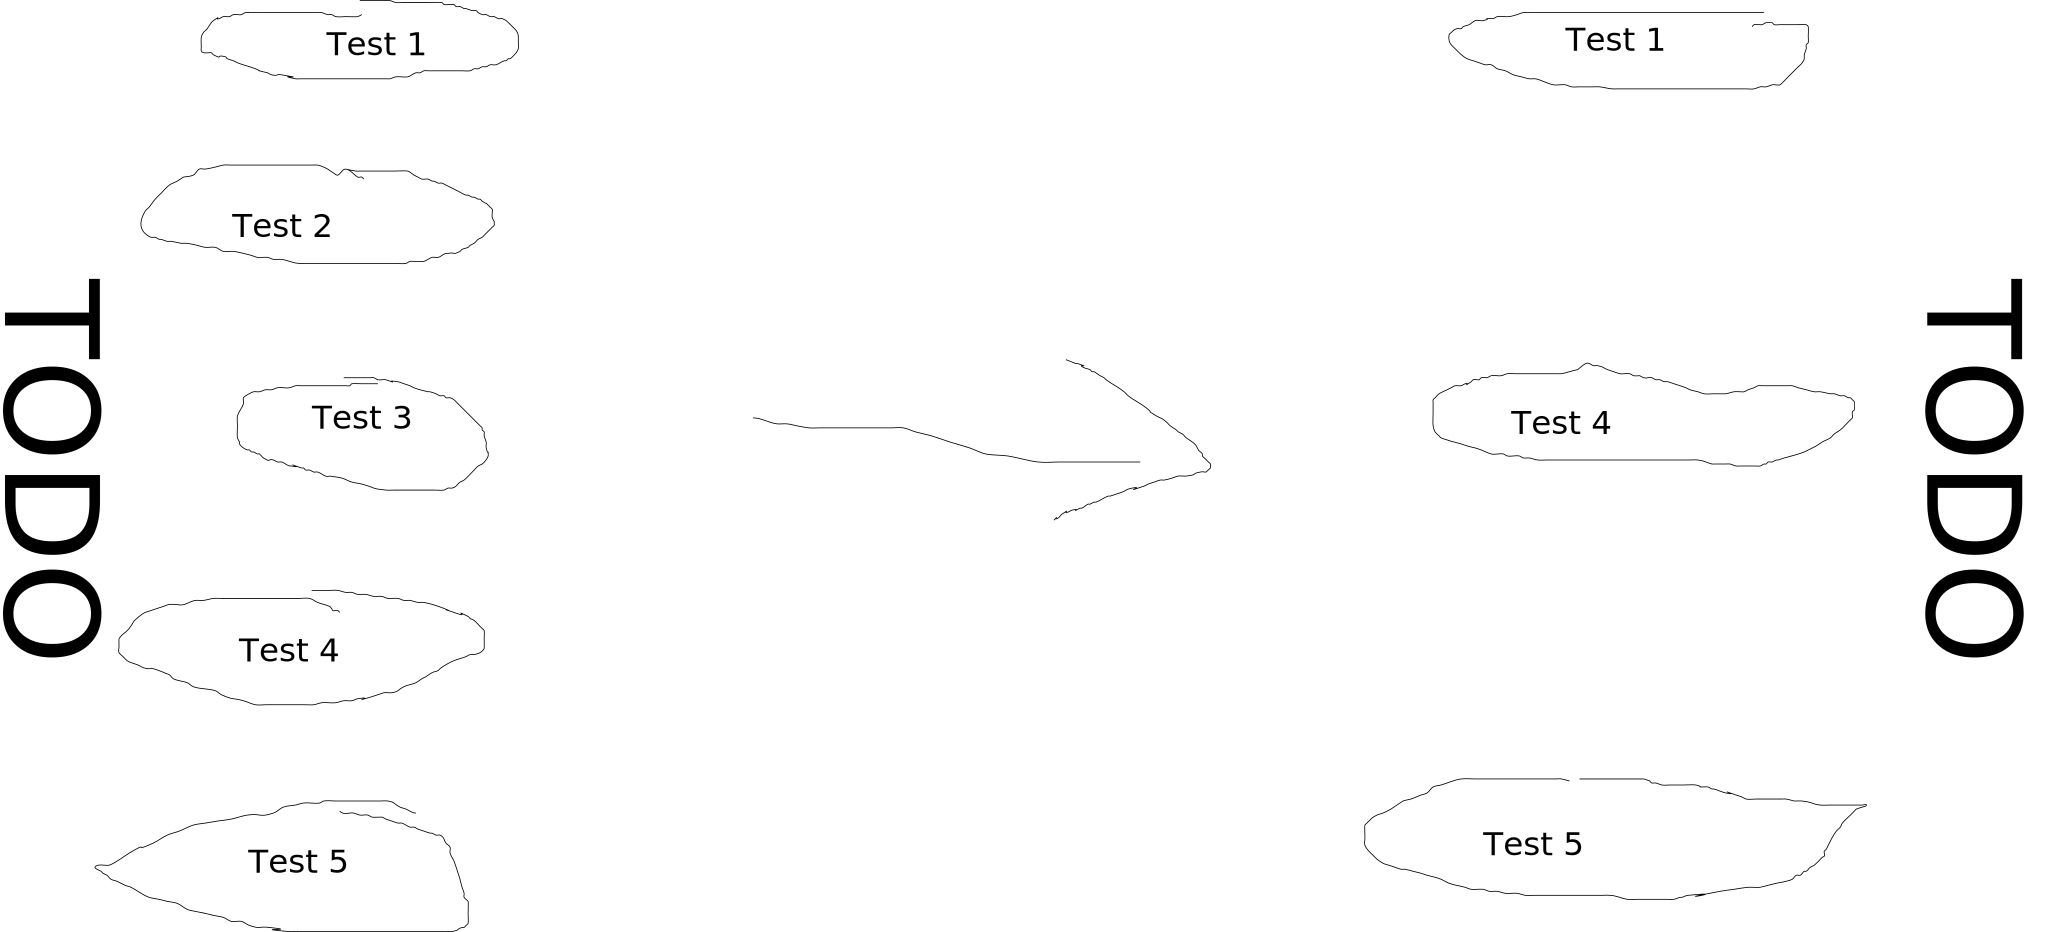
\includegraphics[width=\textwidth]{assets/tikz/approach-tsm.tikz}
	\caption{\tsm{}.}
	\label{fig:tsm}
\end{figure}